\documentclass{article}
\usepackage{graphicx}
\graphicspath{ {Images/} }
\usepackage[square,sort,comma,numbers]{natbib}
\usepackage{caption}
\RequirePackage{xcolor}
\usepackage{titlesec}
\usepackage{float}
\usepackage[margin=1.0in]{geometry}

\newcommand{\divider}{\rule{\linewidth}{0.5mm}}
\definecolor{tudelft-cyan}{cmyk}{1,0,0,0}
\definecolor{tudelft-black}{cmyk}{0,0,0,1}
\definecolor{tudelft-white}{cmyk}{0,0,0,0}
\definecolor{tudelft-sea-green}{cmyk}{0.54,0,0.32,0}
\definecolor{tudelft-green}{cmyk}{1,0.15,0.4,0}
\definecolor{tudelft-dark-blue}{cmyk}{1,0.66,0,0.4}
\definecolor{tudelft-purple}{cmyk}{0.98,1,0,0.35}
\definecolor{tudelft-turquoise}{cmyk}{0.82,0,0.21,0.08}
\definecolor{tudelft-sky-blue}{cmyk}{0.45,0,0.06,0.06}
\definecolor{tudelft-lavender}{cmyk}{0.45,0.2,0,0.07}
\definecolor{tudelft-orange}{cmyk}{0.02,0.56,0.84,0}
\definecolor{tudelft-warm-purple}{cmyk}{0.58,1,0,0.02}
\definecolor{tudelft-fuchsia}{cmyk}{0.19,1,0,0.19}
\definecolor{tudelft-bright-green}{cmyk}{0.36,0,1,0}
\definecolor{tudelft-yellow}{cmyk}{0.02,0,0.54,0}

\setcounter{secnumdepth}{4}

\begin{document}
	\pagenumbering{roman}
	
	\begin{titlepage}
		\setlength\topsep{0pt}
		\setlength\parskip{0pt}
		\begin{center}
			\divider \\[1cm]
			{ \huge \bfseries Review of Distributed Machine Learning}\\[0.4cm]
			\divider \\[1.5cm]
			Jonathan Katzy, Jeroen Kloppenburg, Joost Verbraeken, Matthijs Wolting
			\vfill
			
			\section{Abstract}
\textbf{Background:} asdf
\textbf{Objective:} We aim to provide an overview of the ...
% RESEARCH QUESTION
% SUB-RESEARCH QUESTIONS
\textbf{Methods:} asdf
\textbf{Results:} asdf
\textbf{Conclusions:} asdf
			
			\begin{minipage}{0.4\textwidth}
				\begin{flushleft} \large
					
\includegraphics[width=2.6in]{logo}
				\end{flushleft}
			\end{minipage}
			\begin{minipage}{0.4\textwidth}
				\begin{flushright} \large
					TU Delft\\
					{\large \today}\\
				\end{flushright}
			\end{minipage}\\[1cm]
		\end{center}
	\end{titlepage}

\newpage
	
	\tableofcontents
	
\newpage
	
\pagenumbering{arabic}
	\section{Introduction}
% Convince the reader that Distributed Machine Learning is significant / important / interesting
% Convince the reader that we shouldn't be completely satisfied with the existing literature on this topic and that our research will address some important limitation or deficiency
% Explain our
	% RESEARCH QUESTION
	% SUB-RESEARCH QUESTIONS
	% ALL OF THEM WELL-MOTIVATED
% Give a hypothesis for them

% Clearly formulated andwell-motivated research question. Main research question split up into sub-questions.
% Very well-structured document. General presentation of the content (text and figures) is very effective. 
% Excellent expressed and formulated report. Document has a smooth flow. Spelling and grammatically error free.

With the ever increasing amount of data created every day and the prevalence of Machine Learning (ML) algorithms in analyzing all this data, a lot of research is being done on the application of Distributed Machine Learning approaches. Because of the many different approaches to dealing with so-called Big Data, we would like to give an overview of the current state-of-the-art of Distributed Machine Learning.

Most Machine Learning algorithms assume that all data can be easily accessed. This is not always the case, as some forms of data are inherently distributed, like transaction information for multinationals, or otherwise too big to store on single machines, like astronomical data. Regular Machine Learning algorithms have to be changed to accommodate for these circumstances to still be able to extract useful information from these datasets.

In this paper, we will give an overview of the current state-of-the-art by going over the different theories and technologies used for Distributed Machine Learning and some of the biggest implementations.
	\section{Results}
% Answer research questions

\subsection{The need for Distributed Machine Learning}
\subsubsection{Alternatives to Distributed Machine Learning}
\paragraph{Long-term sustainability}










\subsection{Underlying technology}
To give you an overview of how Distributed Machine Learning works, we'll give you an abstract framework that includes everything a real implementation should include. We do that by exploiting the three unique properties of Distributed Machine Learning, namely error tolerance, dynamic structural dependency and non-uniform convergence.\cite{Xing16}\\
Our goals include (1) to list regular Machine Learning algorithms that are commonly used in a distributed setting; (2) to find algorithms to determine the best parameters for the former algorithms; (3) to tradeoff computation time with communication and accuracy; and (4) to minimize the amount of bits sent over the network so that the system is no bottlenecked by scarce network bandwidth.\\
Designing a general system in such a way that the regular Machine Learning algorithms can be distributed efficiently is challenging, because every algorithm has its own communication patterns \cite{Jia14}\cite{Newman09}\cite{Rich13}\cite{Smola10}\cite{Takac13}\cite{Tsi12}.

\subsubsection{Machine Learning algorithms}
We'll first look at Machine Learning is done at a single machine before looking at distributing these. We'll only give a brief description of the algorithms because single-node machine learning is not the focus of this paper.


\paragraph{Overview}
Machine Learning algorithm-families that are used in the literature and perform the actual "learning" include:
\begin{itemize}
	\item Graphical models \cite{Wain08}\cite{Kol09}\cite{Xin16}
	\begin{itemize}
		\item Latent Dirichlet Allocation Topic Model \cite{Blei03}
	\end{itemize}
	\item Regularized Bayesian models \cite{Zhu09}\cite{Zhu09-2}\cite{Zhu14}
	\item Nonparametric Bayesian models \cite{Grif05}\cite{Teh06}
	\item Sparse structured models
	\begin{itemize}
		\item Lasso regression (group Lasso)
	\end{itemize}
	\item Large-margin methods
	\item Deep learning
	\item Matrix factorization
	\item Sparse coding
	\item Latent space modeling
	\item Distance metric learning
	\item Non-negative matrix factorization
	\item Principal component analysis
\end{itemize}


\paragraph{Algorithms to find best parameters}
To find the parameters for these algorithms we can use several Machine Learning workhorse implementations that can be re-used across different Machine Learning algorithm-families. These include:
\begin{itemize}
	\item First-order techniques
	\begin{itemize}
		\item Stochastic gradient descent
		\item Stochastic dual coordinate ascent\cite{Shal13}
		\item L-BFGS
		\item Conjugate gradient
	\end{itemize}
	\item Second-order techniques
	\begin{itemize}
		\item Newton descent
		\item Quasi-Newton descent
	\end{itemize}
	\item Coordinate descent
	\item Markov-Chain Monte-Carlo
	\item Variational inference
\end{itemize}


% --------


\subsubsection{Partitioning and distribution algorithms}
Now we'll look the abstraction of the general design for a distributed Machine Learning operating system that executes the Machine Learning workhorses across a wide variety of hardware.


\paragraph{Computation time vs communication vs accuracy}


\paragraph{Scheduling and balancing the workloads}
There are 3 things to take into account when partitioning an ML program in order to parallelize it:\cite{Xing16}\\
\begin{enumerate}
	\item Deciding which tasks go or don' go together in parallel
	\item Deciding the order in which tasks will be executed
	\item Ensuring an even load distribution across the machines
\end{enumerate}


\paragraph{Bridging computation and communication}
Let's look at several ways to efficiently communicate between the nodes taking the interleaving of parallel program computations and inter-worker communication into account. These techniques tradeoff communication overhead (at the top of the list) with fresher updates (at the bottom of the list).
\begin{enumerate}
	\item BSP model
	\item Asynchronous parallel execution
	\item Total Asynchronous Parallel (TAP)
	\item Stale Synchronous Parallel (SSP)
	\item ASP
\end{enumerate}


\paragraph{Communication strategies}
To distribute Machine Learning algorithms we can choose to partition either the data or the model across the machines - referred to respectively as data parallelism and model parallelism \cite{Die12}. These two types of parallelism can be applied at the same time \cite{Xing16}. Data parallelism can be applied to every ML algorithm with an i.i.d. assumption over the data samples, which are most ML algorithms \cite{Xing16}. It partitions the data and assigns it to parallel machines. Model parallelism cannot be applied to most ML algorithms, because the model parameters generally don't have this i.i.d. assumption. It partitions the model parameters and assigns that to parallel machines.\\
There are several communication management strategies\cite{Xing16} used to spread and reduce the amount of data communicated between machines:
\begin{itemize}
	\item To prevent bursts of communication over the network, for example after a mapper is finished, continuous communication is used, for example in the state-of-the-art implementation Bösen\cite{Wei15}.
	
	\item Neural networks are composed out of layers, of which the training by using the back-propagation gradient descent algorithm is highly sequential. Because the top layers of neural networks contain a lot more parameters while it accounts only for a small part of the total computation \cite{Xing16}, WFBP \cite{Zhang17} was proposed to spread the computation and communication out in an optimal fashion.
	
	\item Hybrid communication (HybComm) Because WBFP does not reduce the communication overhead, HybComm \cite{Zhang17} was proposed. Effectively it combines Parameter Servers (PS)\cite{Wei15} with Sufficient Factor Broadcasting (SFB)\cite{Xie15} by being aware of both the mathematical property of neural networks and the structure of computing clusters. See below for more information about PS under Centralized Storage and SFB under Decentralized Storage.
	
\end{itemize}


\paragraph{Network topologies}
There are several network topologies used for Distributed Machine Learning clusters:
\begin{itemize}
	\item \textbf{Trees} AllReduce\cite{Agar14} is an example of a tree-like network topology that provides straightforward parallelization of gradient-based optimization algorithms by accumulating local gradients to obtain a global gradient.\\
	An advantage is that AllReduce is very fast and highly scalable. A disadvantage is that it only works for reduce operations like in MapReduce.
	\begin{minipage}{\linewidth}
		\centering
		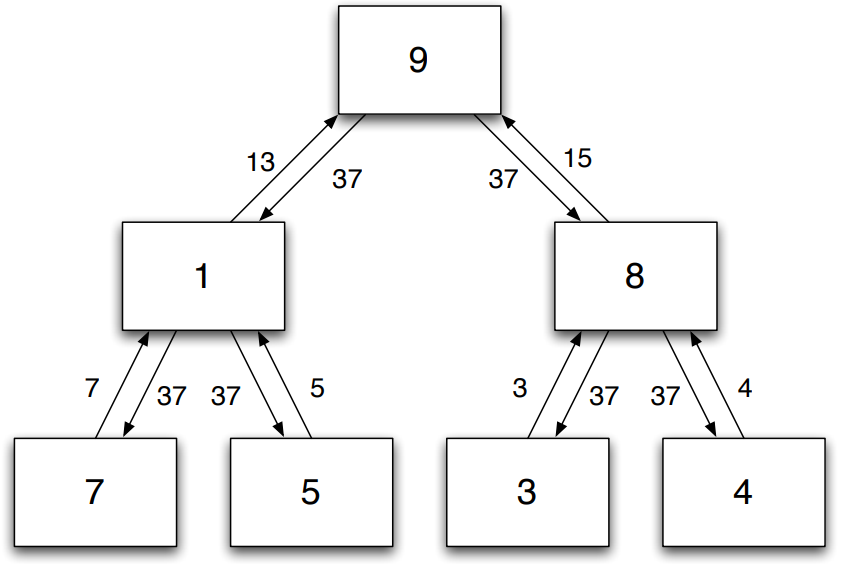
\includegraphics[scale=0.5]{AllReduce.png}
		\captionof{figure}{AllReduce operation. Initially, each node holds its own value. Values are passed up the tree and summed, until the global sum is obtained in the root node (reduce phase). The global sum is then passed back down to all other nodes (broadcast	phase). At the end, each node contains the global sum.}
	\end{minipage}
	\item \textbf{Centralized storage} Centralized storage is used for topologies where a single "master" or "server" node is in the center and many "slave" or "client" nodes communicate only with this master node. A practical implementation of this is the Parameter Server paradigm (PS). Each parameter server keeps a shard of the global model parameters as a key-value store. Each client communicates with the parameter server to read / update the parameters. \\
	An advantage is that all model parameters are in a global shared memory which makes it easy to inspect the model. A disadvantage is that the parameter servers are a bottleneck because they're handling all communication. To partly accommodate this issue, the techniques mentioned under "Bridging computation and communication" are used.
	\item \textbf{Decentralized storage} In contrast to centralized storage, in decentralized storage every worker maintains its own local view of the parameters and the workers communicate directly to each other. An example implementation is a peer-to-peer network where every machine broadcasts everything to all other machines. To reduce the amount of communication between all workers, Sufficient Factor Broadcasting (SFB)\cite{Li13}) was proposed. It Decomposes the parameter matrix \textbf{W} into the outer products of the two vectors \textbf{u} and \textbf{v}: \textbf{ΔW = uv\textsuperscript{T}}. The vectors u and v are \textit{sufficient factors}, meaning that they are sufficient to reconstruct the update matrix \textbf{ΔW}. SFB only broadcasts the sufficient factors and lets the workers reconstruct the updates.\\
	An advantage is that, with SFB, decentralized storage is relatively communication efficient and that there is no centralized bottleneck, making it more scalable.
\end{itemize}










\subsection{Currently used implementations}
\subsubsection{Generic distributed system frameworks}
\subsubsection{Domain-specific implementations}
\subsubsection{Current challenges}










\subsection{Privacy challenges}

	\newpage
	\section{Discussion}
Distributed machine learning is already seeing widespread use, and a variety of findings (both theoretical and practical) have been contributed to the field in recent years.

There is a noticeable gap between state-of-the-art systems that are found in traditional scientific literature, and implementations that are used in industry. While the scientific community is more focused on the theoretical limitations of distributed machine learning in aspects such as communication complexity and relative accuracy, industry systems have less regard for the theory behind the implentation. A good example of this is found in \citep{DistBelief2012}, which contains statements such as "[t]here is little theoretical grounding for the safety of these operations for nonconvex problems, but in practice we found relaxing consistency requirements to be remarkably effective". Compare this to e.g. \citep{Xing16} and its references, in which findings are evaluated within the context of theoretical optimality.

Practical application of distributed artificial neural networks is especially prevalent. State-of-the-art ANNs for complex conditional applications, such as the one described by \citet{Shazeer2017}, require optimizing tens of billions of parameters through tens of billions of samples, and make use of systems such as Tensorflow\citep{Tensorflow2015}\citep{Tensorflow2016} to distribute this process. Even networks of this scale, however, are generally trained on relatively small clusters (less than 100 machines) of powerful multi-GPU nodes. In comparison, computations on Google's deployment of MapReduce\citep{MapReduce} often use thousands of commodity worker machines.

The scale at which distributed ML currently occurs suggests one of two things: either effective ML models do not yet exist that can be efficiently distributed at big data scale, or current distribution methods have not advanced enough yet to support large-scale distributed ML. Improving either of these aspects is beneficial to the other: ML models that are more easily distributed require less advanced distribution mechanisms, whereas more versatile distribution mechanisms can compensate for less efficient ML algorithms. Which strategy will prove simpler to apply is not clear.
	\newpage
	\section{Conclusion}
This paper reviews the current state-of-the-art of Distributed Machine Learning. To answer this main research question, all sub-research questions are answered:
\begin{itemize}
	\item \textbf{What are the advantages of Distributed Machine Learning over (centralized) Machine Learning?}
	\begin{itemize}
		\item \textbf{Which alternatives exist to Distributed Machine Learning?} We discussed several ways to learn from huge amounts of data, including the use of specialized hardware (such as ASICs) and increased computation power per computer (as seen in e.g. the Epiphany architecture)
		\item \textbf{How likely are they to remain sufficient for emerging applications?} While Distributed Machine Learning will provide the highest amount of power in the future because it scales in the best case almost horizontally, alternatives may remain in use for simpler tasks that are too heavy to run on an ordinary machine, but too lightweight for a full Distributed Machine Learning cluster.
	\end{itemize}
	\item \textbf{What technology is used for Distributed Machine Learning?} We created an overview of the algorithms that a general Distributed Machine Learning could use and how they relate to each other:
	\begin{itemize}
		\item \textbf{What algorithms and with which parameters are used to perform the actual Machine Learning?} We divided ML algorithms into categories based on the type of feedback given to the algorithm, its goal, its type and its method.
		\begin{itemize}
			\item \textbf{What algorithms are used to find the best parameters for the algorithms?} We listed several "workhorse" algorithms that optimize the parameters for ML algorithms, categorized as first-order techniques, second-order techniques, coordinate descent, Markov-Chain Monte Carlo, and Variational inference.
			\item \textbf{What algorithms are used to perform the Machine Learning?} For every category, this paper lists several ML methods, with the notable mention of Artificial Neural Networks (ANNs) and Ensemble Learning.
		\end{itemize}
		\item \textbf{How can these algorithms be partitioned and distributed across a wide variety of hardware?} To partition and distribute Machine Learning, there are 5 sub-research questions that need to be answered:
		\begin{itemize}
			\item \textbf{What is the trade-off between computation time VS communication VS accuracy?} Dependent on the characteristics of the dataset and the model being trained, communication can become the bottleneck that limits the level of accuracy that can be achieved by greatly reducing the computation time with more communication.
			\item \textbf{How to schedule and balance the workloads?} To schedule and balance the workloads, we have to take 3 important decisions: which tasks go or don't go in parallel? What is the order in which tasks will be executed? How do we ensure an even load distribution across the machines?
			\item \textbf{How to bridge computation and communication?} There's a trade-off between correct model convergence and faster updates. BSP and SSP focus on correct model convergence but have a lot of communication overhead because of synchronization barriers. ASP is very communication efficient, but is hard to choose the best parameters for. BAP / TAP are also very communication efficient but provide slow or even incorrect model convergence.
			\item \textbf{What strategies can be used to optimize communication overhead?} To prevent bursts of communication, continuous communication is used. WBFP balances computation and communication for Neural Networks optimally and to reduce its communication overhead Hybrid Communication was proposed.
			\item \textbf{What network topologies exist to partition the computing cluster?} There are 3 main network topologies: trees, centralized storage and decentralized storage. Trees are used by AllReduce for to obtain efficiently a global gradient. Centralized Storage is implemented by the Parameter Server paradigm and results in a scalable setting of which the global shared memory is easy to inspect. Decentralized storage is implemented in peer-to-peer networks that provide, in combination with Sufficient Factor Broadcasting, a communication efficient and very scalable environment.
		\end{itemize}
	\end{itemize}
	\item \textbf{What are the currently used implementations?} Many Distributed Machine Learning frameworks are built on top of a framework that manages the large amounts of data (Big Data). GFS is the file system used by Google to handle Big Data, and inspired the creation of an open-source alternative (called HDFS), which is the industry standard for storing big data. On top of GFS / HDFS, several data processing frameworks are built, including MapReduce and Hadoop (which process data using the Bulk-Synchronous Processing (BSP) paradigm), and Apache Spark (which can run more advanced programs than MapReduce tasks, and operate entirely in memory).
	\begin{itemize}
		\item \textbf{Which domain-specific implementations exist?}
		Domain-specific implementations can be categorized by the architecture they use. The two major architectures are synchronous and asynchronous Stochastic Gradient Descent (SGD), which each strike a different balance between raw efficiency and fault-tolerance. Some hybrid architectures also exist, with the purpose of leveraging the benefits of either style, but these have not seen the same level of real-world application as their non-hybrid counterparts.
		\item \textbf{What are the current challenges with these implementations?}
		\begin{itemize}
			\item \textbf{What are the performance challenges?} In the past, companies have had to increase the number of machines quadratically to achieve a linear increase in performance. With state-of-the-art machine learning systems like Tensorflow, the scaling is still below 75\%, although synchronous SGD-based frameworks can achieve almost linear scaling at small cluster sizes.
			\item \textbf{What are the fault-tolerance challenges?} At large cluster sizes, the probability of a single node failure is high. This has lead to High-Performance Computing-inspired patterns, such as checkpointing. In practice, companies have to balance performance with fault tolerance, because no good hybrid approaches have been developed yet.
			\item \textbf{What are the privacy challenges?} Taking political decision into account, some data is not allowed to move past country borders or even move at all. Distributed Ensemble Models, Parameter Server-based systems, and statistical noise offer improved privacy, but perfect privacy is not focused on by current frameworks.
		\end{itemize}
	\end{itemize}
\end{itemize}

	
\newpage

\pagenumbering{alph}
	
	\bibliography{myrefs}
	\bibliographystyle{apalike}

\newpage

	\section{Appendix A - Research Questions}
We answered in this paper the following research question:\\
\textbf{Key question: What is the current state-of-the-art of distributed machine learning?}
\begin{itemize}
	\item \textit{We ask this very broad question to assess to entire topic of Distributed Machine Learning, as required by the course.}
	\item Why do we want or need Distributed Machine Learning opposed to (centralized) Machine Learning?
	\begin{itemize}
		\item \textit{We ask this question to motivate the need to use Distributed Machine Learning. Machine Learning is already practiced widely, and through this question we will research if it is actually necessary to distribute this machine learning.}
		\item Which alternatives exist to Distributed Machine Learning?
		\begin{itemize}
			\item \textit{We ask this question to discover if there are any alternatives to Distributed Machine Learning that we need to take into account. If there are none and the answer to the former question (do we need Distributed Machine Learning) is true, we only need to focus on Distributed Machine Learning. If not, we will recommend to which extent Distributed Machine Learning should be applied, in part based on the result of the next subquestion:}
			\item How likely are they to remain sufficient for emerging applications?
			\begin{itemize}
				\item \textit{We ask this question to assess whether the alternatives to Distributed Machine Learning will remain sufficient in the future. If not, that might guide us to focus research efforts on Distributed Machine Learning, which should be able to remain sufficient for emerging application, as will be answered in Why we want / need Distributed Machine Learning.}
			\end{itemize}
		\end{itemize}
	\end{itemize}
	\item What technology is used for Distributed Machine Learning?
	\begin{itemize}
		\item \textit{We ask this question to gain an understanding of how Distributed Machine Learning works, and what the differences in its implementations are. When researchers want to propose new and better methods for Distributed Machine Learning, they have to know first about how the current methods work, or at least have an overview of the current methods and references that provide a more thorough explanation.}
		\item What algorithms (and with which parameters) are used to perform the actual machine learning?
		\begin{itemize}
			\item \textit{We ask this question to learn how the current state-of-the-art Machine Learning algorithms compute their output from their input and parameters. This is important, because, as we’ll explain in this section, it is desirable to be able to distribute existing Machine Learning algorithms.}
			\item What algorithms are used to find the best parameters for the algorithms?
			\begin{itemize}
				\item \textit{We ask this question because bare Machine Learning algorithms are nearly useless without good parameters. Therefore, we want to find methods that approximate or (hopefully) find optimal parameter values.}
			\end{itemize}
			\item What algorithms are used to perform the machine learning?
			\begin{itemize}
				\item \textit{We ask this question to learn how the current state-of-the-art Machine Learning algorithms work. This is important, because, as we’ll explain in the parent question, it is desirable to being able to distribute existing Machine Learning algorithms.}
			\end{itemize}
		\end{itemize}
		\item How can we partition and distribute these algorithms across a wide variety of hardware?
		\begin{itemize}
			\item \textit{We ask this question because, without this question, this paper would essentially be about non-distributed Machine Learning algorithms (as opposed to Distributed Machine Learning algorithms). We want to know how to partition and distribute the Machine Learning algorithms to accommodate the answer to the question Why do we want / need Machine Learning (which will, as will be explained in the paper, motivate the need for Distributed Machine Learning).}
			\item What is the trade-off between computation time, communication, and accuracy?
			\begin{itemize}
				\item \textit{We ask this question because you cannot perform well on all 3 of these, as will be explained in the paper. Therefore, we want to research where the sweet spot is. This is important, because the sweet spot can be defined as the ultimate combination between these 3 factors, which provides us with an optimal result.}
			\end{itemize}
			\item How to schedule and balance the workloads?
			\begin{itemize}
				\item \textit{We ask this question because we want to know when and where to execute what code, in order to achieve acceptable distributed performance.}
			\end{itemize}
			\item How to bridge computation and communication?
			\begin{itemize}
				\item \textit{We ask this question because Distributed Machine Learning algorithms need to communicate in order to agree on a common answer. Therefore, we want to research how to interleave parallel program computations and inter-worker communication, and gain insight on how to optimize distributed workloads.}
			\end{itemize}
			\item What strategies can be used to optimize communication overhead?
			\begin{itemize}
				\item \textit{We ask this question because communication is generally very slow. Therefore, we want to research which techniques exist to improve performance in regard to communication.}
			\end{itemize}
			\item What network topologies exist to partition the computing cluster?
			\begin{itemize}
				\item \textit{We ask this question because there are many ways to partition machines within computing clusters in regard to the destination of outgoing network packets from machines. We want to know when to use which of these network topologies for optimal performance.}
			\end{itemize}
		\end{itemize}
	\end{itemize}
	\item What are the currently used implementations?
	\begin{itemize}
		\item \textit{We ask this question because the former sections only gave an abstract overview of techniques that are used in current implementations. To contribute to the field, however, it is also important to improve existing implementations. To enable this, we want to get an overview of currently existing implementations and how they compare against each other.}
		\item Which implementations make use of generic distributed systems frameworks? (Hadoop, Spark, GraphLab, etc.)
		\item Which domain-specific implementations exist? (Tensorflow, MXNet, CNTK, etc.)
		\begin{itemize}
			\item \textit{We ask this question because most domain-specific implementations distinguish themselves from more generic systems quite obviously. There’s optimizations that only make sense when exploiting the unique properties of e.g. a neural network, and design considerations that are easier to make with known requirements on communication and computation.}
		\end{itemize}
		\item What are the current challenges with these implementations?
		\begin{itemize}
			\item \textit{We ask this question because there are bound to be areas of improvement in each of the aforementioned systems. Whether this is because of unsolved problems, or because all existing systems make severe trade-offs, it is interesting to see which areas of focus could be considered when developing a new framework.}
			\item Performance challenges?
			\begin{itemize}
				\item \textit{We ask this question because performance is a core motivation for the use of Distributed Machine Learning. If it is very hard to achieve high performance with existing implementations, they do not offer a solution to the problems they mean to solve.}
			\end{itemize}
			\item Fault-tolerance challenges?
			\begin{itemize}
				\item \textit{We ask this question to learn what the impact on the training process is of slow communication or a node failure (the likelihood of which increases with cluster size).}
			\end{itemize}
			\item Privacy challenges?
			\begin{itemize}
				\item \textit{We ask this question because possible sensitive data of users is frequently communicated between many different machines in a distributed system. Through patterns in the communication streams, sensitive data may leak unintentionally. We therefore want to assess what the risks and consequences of this are, and how we can prevent it from happening.}
			\end{itemize}
		\end{itemize}
	\end{itemize}
\end{itemize}


\end{document}
